\section{INTRODUCTION}

\subsection{The Convergence of Sensing and Communication: A 6G Imperative}

The escalating complexity of the electromagnetic environment has intensified demands for ultra-reliable wireless connectivity, driving significant interest in Integrated Sensing and Communication (ISAC) systems \cite{O_ISAC_070}. This integrated approach enables ultra-efficient spectrum utilization and significantly reduces hardware costs, and more importantly, establishes a foundational framework for achieving seamless connectivity in future wireless networks \cite{O_ISAC_070}. ISAC has now emerged as a core enabler in 6G networks and is recognized as one of the six key usage scenarios by both the ITU-R IMT-2030 framework \cite{O_ISAC_162} and 3GPP \cite{O_ISAC_162}, spanning the coexistence, cooperation, and co-design of communication and sensing functionalities \cite{O_ISAC_070}.

The intelligence of future society necessitates an immediate requirement for ultra-high-speed communication and ultra-resolution sensing in the 6G era \cite{O_ISAC_016}. As intelligent applications---including robot navigation, augmented reality, autonomous driving, and human--machine interaction---continue to proliferate, these emerging services require the capability of highly-reliable wireless communication and high-accuracy environment sensing simultaneously \cite{O_ISAC_351}. Wireless communication frequency bands are gradually transitioning to higher frequency ranges---encompassing millimeter-wave (mmWave) and terahertz (THz)---to fulfill the ultra-high data rate requirements of this vision. \textbf{Despite significant progress in RF-based ISAC}, the conventional independent design of communication and sensing systems generally occupies disjoint spectral resources, profoundly aggravating spectrum congestion \cite{O_ISAC_351}. Moreover, using traditional all-electronic approaches to generate mmWave or THz signals will inevitably encounter challenges such as high complexity and \textbf{bandwidth limitation}, which will increase the system costs significantly \cite{O_ISAC_286}. To the best of our knowledge, conventional RF-ISAC systems face three fundamental constraints:

\begin{enumerate}
    \item \textbf{Spectrum Congestion}: With the rapid advances of wireless mobile devices, RF communication and sensing systems face challenges such as spectrum congestion, limited bandwidth, and susceptibility to electromagnetic interference \cite{O_ISAC_068}. The exponentially growing demand for mobile data, coupled with stringent sensing resolution requirements of emerging applications (holographic telepresence, digital twins, autonomous navigation), has created significant pressure on the congested RF spectrum \cite{O_ISAC_161}.
    \item \textbf{Limited Resolution and Bandwidth}: The spatial resolution achievable in the mmWave band is fundamentally limited to approximately centimeter-level, insufficient for millimeter-precision applications \cite{O_ISAC_021}. Furthermore, RF-ISAC systems commonly suffer from \textbf{spectrum scarcity, high power consumption, and limited sensing capabilities} \cite{O_ISAC_203}.
    \item \textbf{Hardware Constraints}: Purely electrical THz systems struggle to achieve the wide bandwidth and flexible reconfigurability demanded by 6G \cite{O_ISAC_070}. The construction of mmWave/THz ISAC systems using purely electrical means is associated with bandwidth and frequency adjustability limitations that increase overall system complexity \cite{O_ISAC_286}.
\end{enumerate}

\textbf{Recent advances in photonic THz techniques have opened new opportunities} for transcending these RF limitations. \textbf{Optical Integrated Sensing and Communication (O-ISAC)} has emerged as a transformative paradigm that unifies perception, transmission, and processing on optical carriers \cite{O_ISAC_021}. \textbf{Fig. 1} illustrates this paradigm evolution through three distinct phases: \textbf{(A)} the fundamental spectral and bandwidth constraints of conventional RF-ISAC; \textbf{(B)} the transformative opportunities of the optical domain, leveraging the 28.3--845 THz spectrum to enable Tbps-class capacity and mm-scale resolution; and \textbf{(C)} the unified taxonomy of this review, which branches O-ISAC into fiber-based, wireless (FSO/THz), and VLC modalities. Our systematic analysis of \textbf{220 peer-reviewed O-ISAC studies (2020--2025)} reveals that optical ISAC prototypes have pushed these limits: photonic-terahertz integration has achieved \textbf{120 Gbps wireless throughput with 2.5 mm sensing resolution} \cite{O_ISAC_105}, corresponding to $\text{CRQ}_{\Delta} \approx 4.8\times10^{13}$ bps/m \cite{O_ISAC_105}. Earlier photonic sub-THz demonstrations report $\text{CRQ}_{\Delta}$ on the order of $1.0\times10^{13}$ bps/m \cite{O_ISAC_016}.

\begin{figure}[htbp]
    \centering
    
\includegraphics[width=\linewidth]{figures/fig1.png}
    \caption{The O-ISAC paradigm evolution. (A) RF-ISAC systems in sub-6 GHz/mmWave bands often face deployment-constrained spectrum and hardware limits, motivating a transition toward photonic carriers to pursue Tbps-class capacity and mm-scale sensing targets. (B) Optical-ISAC leverages the broad photonic spectrum ($\approx$28.3--845 THz), with implementations clustering in operational windows (telecom for fiber and NIR/visible/photonic-THz for wireless). The review taxonomy branches Optical-ISAC into fiber-based, free-space/photonic-THz, and VLC/LiFi modalities, each characterized by distinct signal models and dominant impairments.}
    \label{fig:fig1}
\end{figure}

Recent photonic and fiber demonstrations illustrate the rate--resolution frontier: a 275 GHz LFM-QAM system reports 120 Gbps with a (two-way) bandwidth-limited range resolution $\Delta r_{\min} \approx 2.5$ mm, yielding $\text{CRQ}_{\Delta} := R / \Delta r_{\min} = 4.8\times10^{13}$ bps/m (equivalently 480 Gbps/cm) \cite{O_ISAC_105}; a D-band sub-THz FDM link delivers 251.03 Gbps with $\Delta r_{\min}=2.5$ cm \cite{O_ISAC_016}; and co-wavelength DAS/DSM over a 38 km seven-core fiber sustains 241.85 Tb/s while sensing 0.1 Hz vibrations with 20 m spatial granularity \cite{O_ISAC_046}. These exemplars highlight the bandwidth advantages of optical carriers and motivate a systematic question.

\textit{These demonstrations motivate a fundamental question: What unique properties of the optical domain enable such performance gains, and how can these advantages be systematically exploited for next-generation ISAC systems?} To address this question, we now examine the physical foundations that position the optical spectrum as the natural substrate for high-performance ISAC.

Table I previews the axis-based comparison of related review- and survey-style works discussed in Section I-D.

\begin{table}[htbp]
\caption{Axis-Based Comparison of This Review with Existing Related Review- and Survey-Style Works}
\label{tab:axis_comparison}
\centering
\footnotesize
\setlength{\tabcolsep}{2pt}
\renewcommand{\arraystretch}{1.1}
\begin{tabularx}{\textwidth}{@{}C{1.15cm}C{0.75cm}C{0.65cm}Y C{0.85cm}L{1.35cm}C{0.8cm}C{0.85cm}C{0.95cm}C{0.85cm}C{0.85cm}@{}}
\toprule
\thead{Ref.} & \thead{Year} & \thead{Tier} & \thead{Modality\\Scope} & \thead{Int.\\Depth} & \thead{Method} & \thead{Tax.} & \thead{Metrics} & \thead{Bench.} & \thead{Transfer} & \thead{Enablers} \\
\midrule
\cite{O_ISAC_161} & 2025 & 2 & $\circ$ / $\circ$ / $\circ$ / $\circ$ & $\bullet$ & Rev. & $\oslash$ & -- & -- & -- & -- \\
\cite{O_ISAC_068} & 2023 & 2 & $\circ$ / $\circ$ / $\bullet$ / $\circ$ & $\bullet$ & Narr. & -- & -- & -- & -- & -- \\
\cite{O_ISAC_327} & 2024 & 2 & $\circ$ / $\circ$ / $\bullet$ / $\circ$ & $\oslash$ & Surv. & $\oslash$ & -- & -- & -- & -- \\
\cite{O_ISAC_006} & 2024 & 2 & $\bullet$ / $\circ$ / $\circ$ / $\circ$ & $\oslash$ & Rev. & -- & $\oslash$ & -- & -- & -- \\
\cite{O_ISAC_368} & 2023 & 2 & $\bullet$ / $\circ$ / $\circ$ / $\circ$ & $\oslash$ & Rev. & -- & -- & -- & -- & -- \\
\cite{O_ISAC_021} & 2023 & 2 & $\circ$ / $\bullet$ / $\circ$ / $\circ$ & $\bullet$ & Tut. & $\oslash$ & $\oslash$ & -- & -- & $\oslash$ \\
\cite{O_ISAC_070} & 2025 & 2 & $\circ$ / $\circ$ / $\circ$ / $\bullet$ & $\bullet$ & Narr. & $\oslash$ & -- & -- & -- & -- \\
\cite{O_ISAC_163} & 2025 & 2 & $\circ$ / $\circ$ / $\circ$ / $\circ$ & $\bullet$ & Surv. & $\oslash$ & -- & -- & $\oslash$ & $\bullet$ \\
\cite{O_ISAC_303} & 2024 & 1 & $\circ$ / $\circ$ / $\bullet$ / $\circ$ & $\bullet$ & Rev. & $\oslash$ & $\oslash$ & -- & -- & -- \\
\textbf{This Review} & \textbf{2026} & \textbf{--} & \textbf{$\bullet$ / $\bullet$ / $\bullet$ / $\bullet$} & \textbf{$\bullet$} & \textbf{PRISMA} & \textbf{$\bullet$} & \textbf{$\bullet$} & \textbf{$\bullet$} & \textbf{$\bullet$} & \textbf{$\bullet$} \\
\bottomrule
\end{tabularx}
\end{table}

\textit{Legend: $\bullet$ = strong/explicit (Score 1); $\oslash$ = partial/within-modality (Score 0.5); -- = absent (Score 0); $\circ$ = out-of-scope. Modality Scope uses ($\circ$/$\oslash$/$\bullet$) only. F = Fiber, FSO = Free-Space Optics, VLC = Visible Light, THz = Photo-THz. THz denotes photonic-THz / optical--THz bridging O-ISAC (not generic RF THz-ISAC hardware surveys).}
\textit{Scoring Criteria: Symbols are mapped via $s_a(p) \in \{0, 1/2, 1\}$ to $\{--, \oslash, \bullet\}$ based on evidence strength: \textbf{$\bullet$} = Systematic/Cross-modal (e.g., unified taxonomy, defined benchmark suite); \textbf{$\oslash$} = Partial/Single-modality; \textbf{--} = Absent/Unaddressed.}

\subsection{The Optical Opportunity: A Vast and Untapped Frontier}

Moving from the RF spectrum crisis to a potential solution, the optical domain---spanning the infrared (IR), visible, and ultraviolet bands---presents an opportunity of transformative scale. While RF-ISAC operates within a congested spectrum below 300 GHz, O-ISAC nominally spans approximately \textbf{28.3 THz to 845 THz} (corresponding to wavelengths from 355 nm to 10.6 $\mu$m), though practical systems cluster within established atmospheric transmission windows and fiber telecom bands \cite{O_ISAC_021}. In this review, Photo-THz O-ISAC refers to photonics-enabled architectures where optical carriers are used for generation/LO/distribution, while the wireless propagation carrier resides in the sub-THz/THz band---thus forming an optical--THz bridging modality. This section elucidates the fundamental physical advantages that position the optical domain as the natural substrate for next-generation ISAC systems.

\subsubsection{Quantitative Comparison: RF-ISAC vs. O-ISAC}

To ground our analysis in empirical data, Table II presents a head-to-head comparison between RF-ISAC modalities (WiFi, mmWave) and O-ISAC, synthesized from our systematic corpus analysis of 220 peer-reviewed studies \cite{O_ISAC_021}.

\begin{table}[htbp]
\caption{RF-ISAC vs. O-ISAC Performance Comparison \cite{O_ISAC_021}}
\label{tab:performance_comparison}
\centering
\footnotesize
\setlength{\tabcolsep}{3pt}
\renewcommand{\arraystretch}{1.12}
\begin{tabularx}{\textwidth}{@{}L{2.4cm}YYY@{}}
\toprule
\thead{Characteristic} & \thead{RF-ISAC\\(Sub-6 GHz / mmWave)} & \thead{Wireless O-ISAC\\(FSO / VLC / Photo-THz)} & \thead{Wired O-ISAC\\(Fiber Sensing)} \\
\midrule
\textbf{Carrier Frequency} & 2.4--100 GHz & 0.1--10 THz (Photo-THz) + 28.3--845 THz (FSO/VLC) & 193 THz (C-Band / L-Band) \\
\textbf{Physics Model} & Diffuse Multipath (Rich) & Line-of-Sight (LoS) Dominated & Guided Mode (Low Loss, Dispersive) \\
\textbf{Signal Type} & Complex (I/Q) & Real (IM/DD) or Complex (Coherent FSO) & Complex (Coherent Phase/Polarization) \\
\textbf{Key Impairments} & Interference, Multi-path Fading & Ambient Light, Turbulence, Pointing Error & Nonlinearity (Kerr), PMD, Phase Noise \\
\textbf{Sensing Task} & Radar (Range/Doppler) & Localization, Gesture, Surface Profiling & DAS (Vibration), Strain, Temperature \\
\textbf{Peak Data Rate} & $\sim$10--20 Gbps & \textbf{$\sim$100--120 Gbps} \cite{O_ISAC_105} & \textbf{$>$ 200 Tbps} (Aggregate) \cite{O_ISAC_046} \\
\textbf{Resolution} & cm-level & \textbf{mm-level (2.5 mm)} \cite{O_ISAC_105} & m-level (Spatial) / $n\varepsilon$ (Strain) \\
\bottomrule
\end{tabularx}
\end{table}

\subsubsection{Three Competitive Advantages of O-ISAC}

Drawing from the generalized O-ISAC system architecture proposed in \cite{O_ISAC_021}, we identify three fundamental advantages that differentiate optical approaches from their RF counterparts. \textbf{Fig. 2} provides a technical "zoom-in" on the physical mechanisms underlying these advantages, contrasting optical physics with RF constraints.

\begin{figure}[htbp]
    \centering
    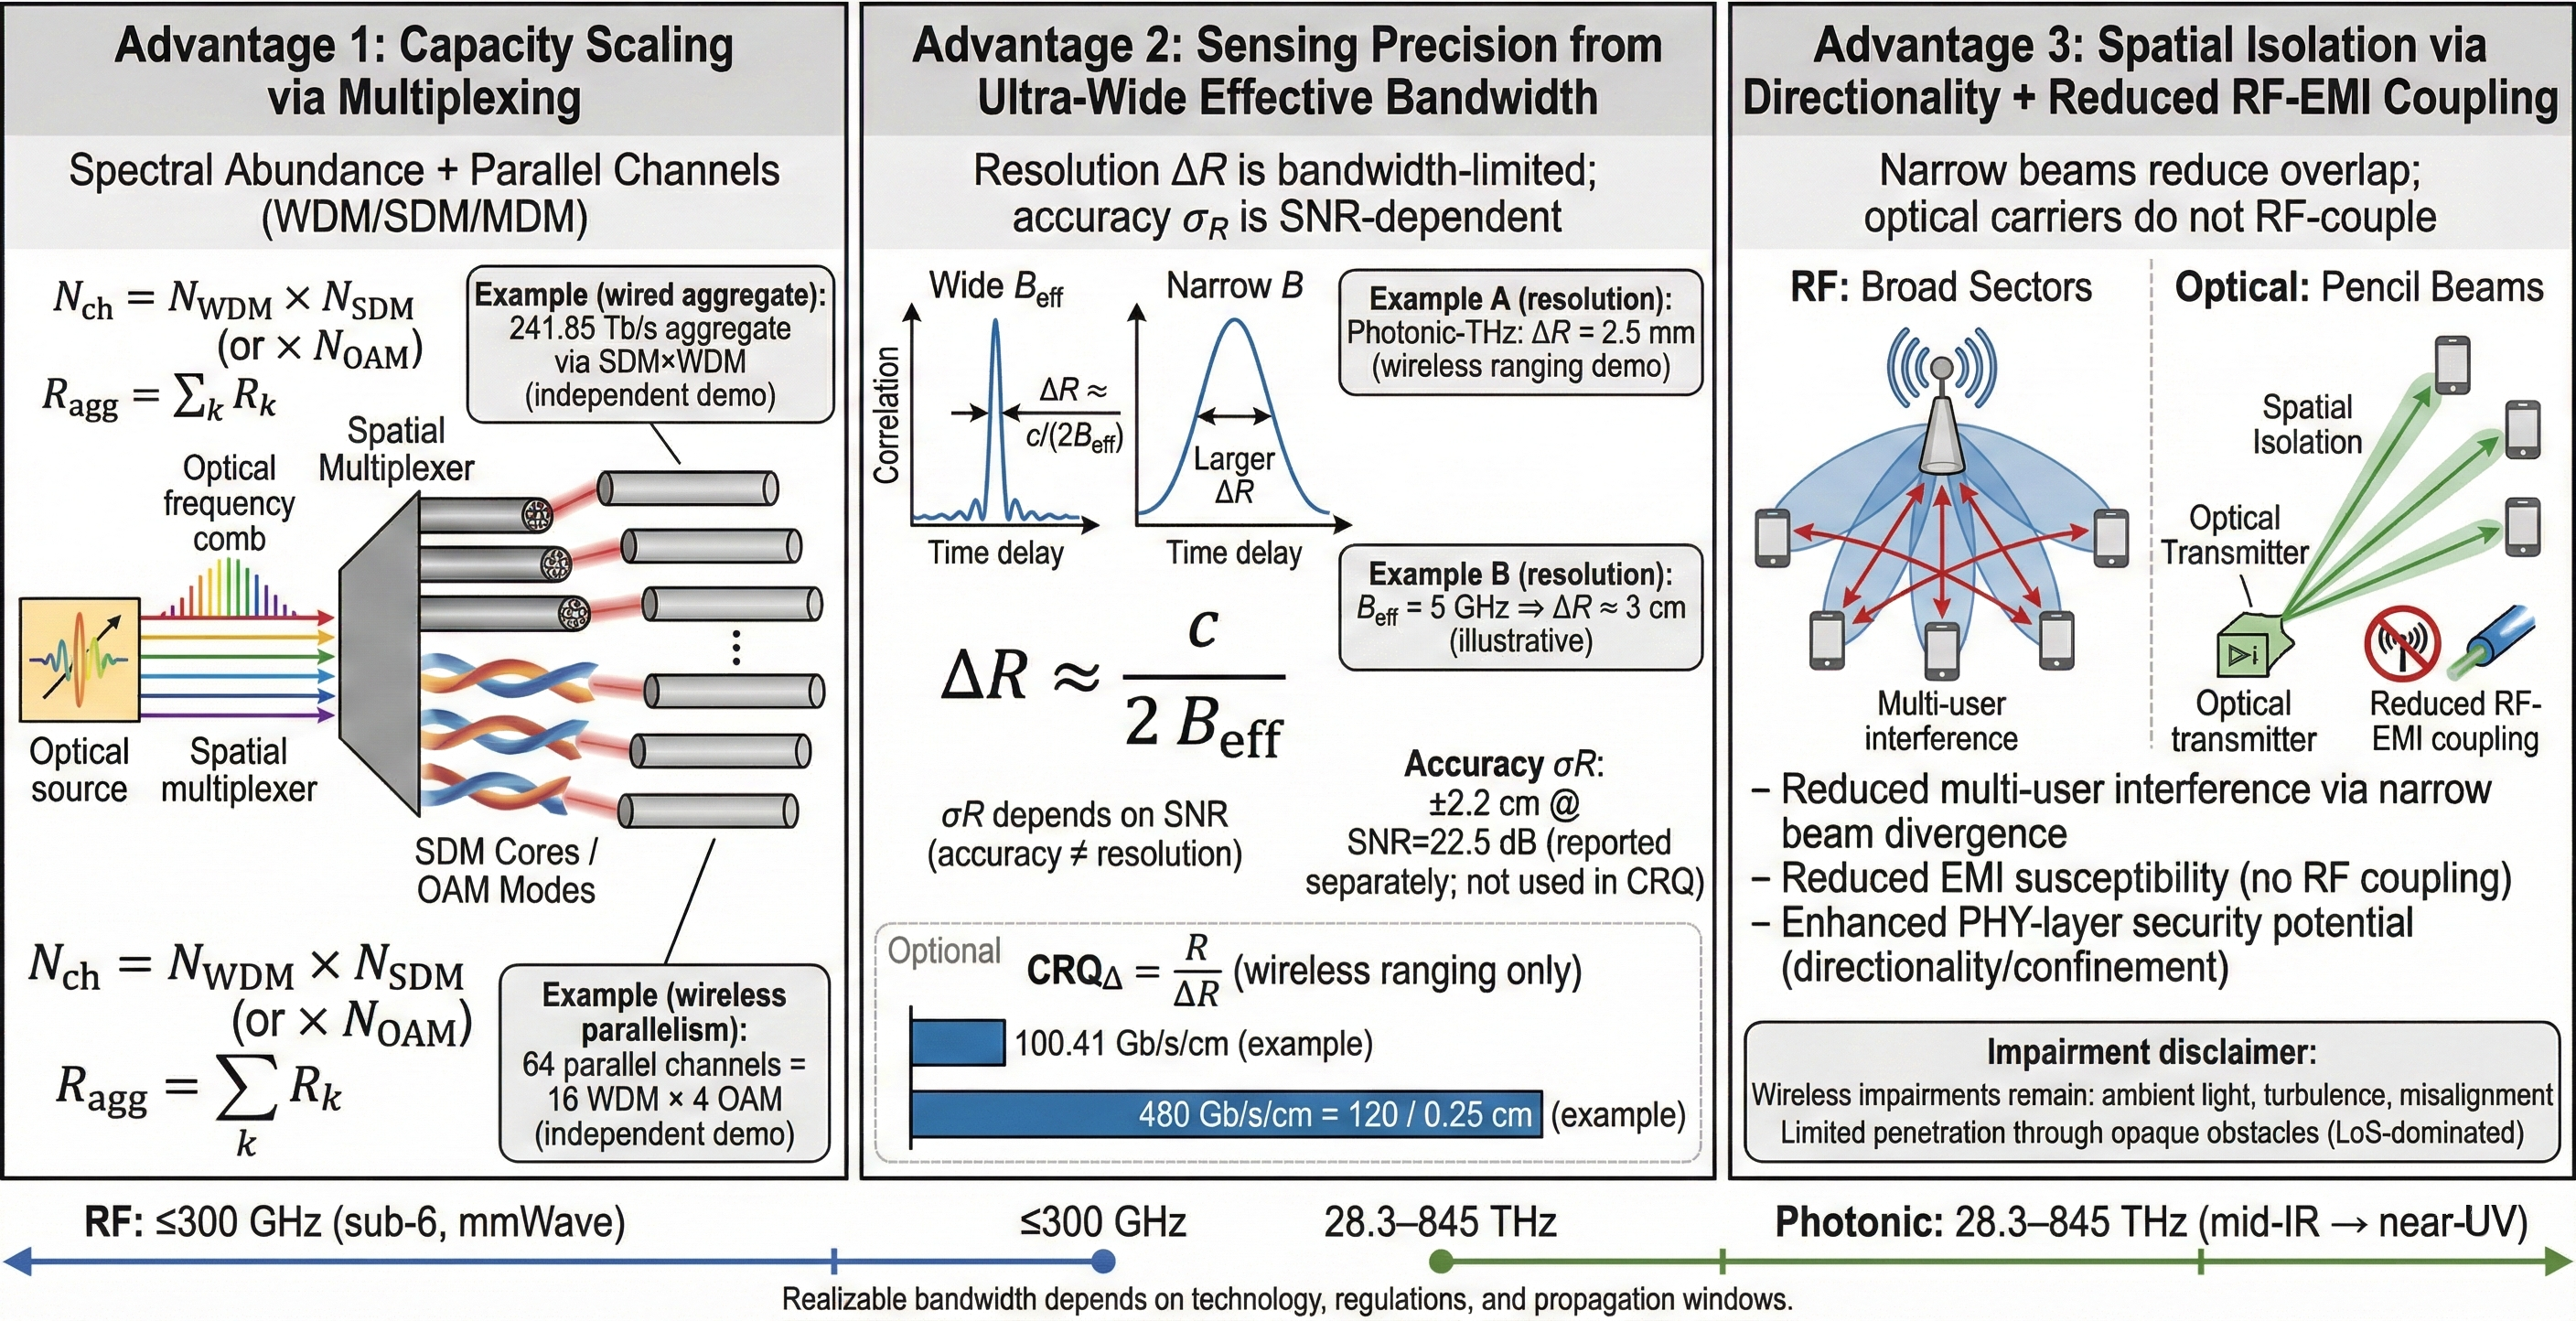
\includegraphics[width=\linewidth]{figures/fig2.png}
    \caption{Physical mechanisms behind the three competitive advantages of O-ISAC. (Left) Capacity scaling is achieved via dense Multiplexing (WDM/SDM), enabling aggregate rates of 241.85 Tb/s (wired) \cite{O_ISAC_046} and dense parallel channels (wireless) \cite{O_ISAC_021}. (Center) Sensing precision is driven by ultra-wide effective bandwidth, enabling wireless range resolution down to $\Delta r_{\min} = 2.5$ mm and $\text{CRQ}_{\Delta}$ of $4.8\times10^{13}$ bps/m (480 Gbps/cm) \cite{O_ISAC_105}. (Right) Spatial isolation is inherent to narrow optical beams, reducing multi-user interference and RF-EMI susceptibility compared to wide RF sectors.}
    \label{fig:fig2}
\end{figure}

\paragraph{Advantage 1: Capacity Scaling Through Spectral Abundance and Multiplexing}
The optical spectrum (spanning \textbf{28.3 THz to 845 THz} \cite{O_ISAC_021}) offers massive resources for dense multiplexing. Unlike RF systems limited by sub-6 GHz blocks, optical carriers support massive parallelism as illustrated in \textbf{Fig. 2 (Left)}:
\begin{itemize}
    \item \textbf{Wireless Parallelism:} Experimental demonstrations of Mode Division Multiplexing (MDM) combined with WDM have realized \textbf{64 parallel channels} (16 wavelengths $\times$ 4 OAM modes) to scale wireless throughput \cite{O_ISAC_021}.
    \item \textbf{Wired Aggregate Capacity:} In the cabled domain, Space Division Multiplexing (SDM) using 7-core fiber has achieved an aggregate capacity of \textbf{241.85 Tbps} (96 WDM channels $\times$ 7 cores) over 38 km \cite{O_ISAC_046}.
\end{itemize}
\textit{These independent demonstrations validate the scalability of optical multiplexing beyond single-link RF limits.}

\paragraph{Advantage 2: Enhancing Sensing Precision via Ultra-Wide Bandwidth}
Range resolution ($\Delta r_{\min}$) is bandwidth-limited in two-way sensing according to $\Delta r_{\min} = v/(2B_{\text{eff}})$ (two-way ranging convention). The ultra-wide bandwidths available in the optical domain enable millimeter-level resolution that is physically difficult for narrowband RF systems to match (\textbf{Fig. 2, Center}):
\begin{itemize}
    \item \textbf{Wireless Ranging:} Photonic-THz systems have demonstrated a \textbf{range resolution of 2.5 mm} alongside 120 Gbps data transmission \cite{O_ISAC_105}.
    \item \textbf{Capacity-Resolution Quotient ($\text{CRQ}_{\Delta}$):} This combination yields $\text{CRQ}_{\Delta} := R / \Delta r_{\min}$ of $4.8\times10^{13}$ bps/m (480 Gbps/cm) for wireless ranging \cite{O_ISAC_105}.
\end{itemize}
\textit{Note: We strictly distinguish bandwidth-limited range resolution ($\Delta r_{\min}$) from SNR-dependent range accuracy ($\sigma_r = \sqrt{\mathbb{E}[(\hat r - r)^2]}$). While fiber DAS achieves meter-level spatial granularity ($\Delta z \approx 20$ m \cite{O_ISAC_046}), its sensing value lies in ultra-sensitive vibration detection rather than high-resolution ranging.}

\paragraph{Advantage 3: Spatial Isolation and Reduced RF-EMI Coupling}
The high directionality of optical beams provides deployment-dependent spatial isolation, significantly reducing Multi-User Interference (MUI) compared to wide-beam RF sectors in clear line-of-sight scenarios \cite{O_ISAC_021}. While wireless O-ISAC links remain susceptible to atmospheric turbulence and ambient light \cite{O_ISAC_003}, their reduced susceptibility to conventional RF Electromagnetic Interference (EMI) and narrow beam divergence (typically on the order of milliradians \cite{O_ISAC_021}) enable dense spatial reuse in deployment scenarios with favorable propagation conditions.

\subsection{Unified O-ISAC Taxonomy}

Having established the physical mechanisms behind the three optical advantages---capacity scaling via multiplexing, bandwidth-limited ranging resolution, and directional spatial isolation---we next formalize the scope of this review. Specifically, the O-ISAC literature does not constitute a single monolithic system class; rather, it clusters into distinct modalities determined by the propagation medium and the associated signal/impairment models. \textbf{Fig. 3} summarizes the resulting evidence-based taxonomy from our PRISMA-compliant 2020--2025 corpus, organizing O-ISAC into four modalities (fiber, free-space optical, VLC/LiFi, and photonic-THz) with their representative operating windows, dominant techniques, and canonical sensing--communication metrics.

\begin{figure}[htbp]
    \centering
    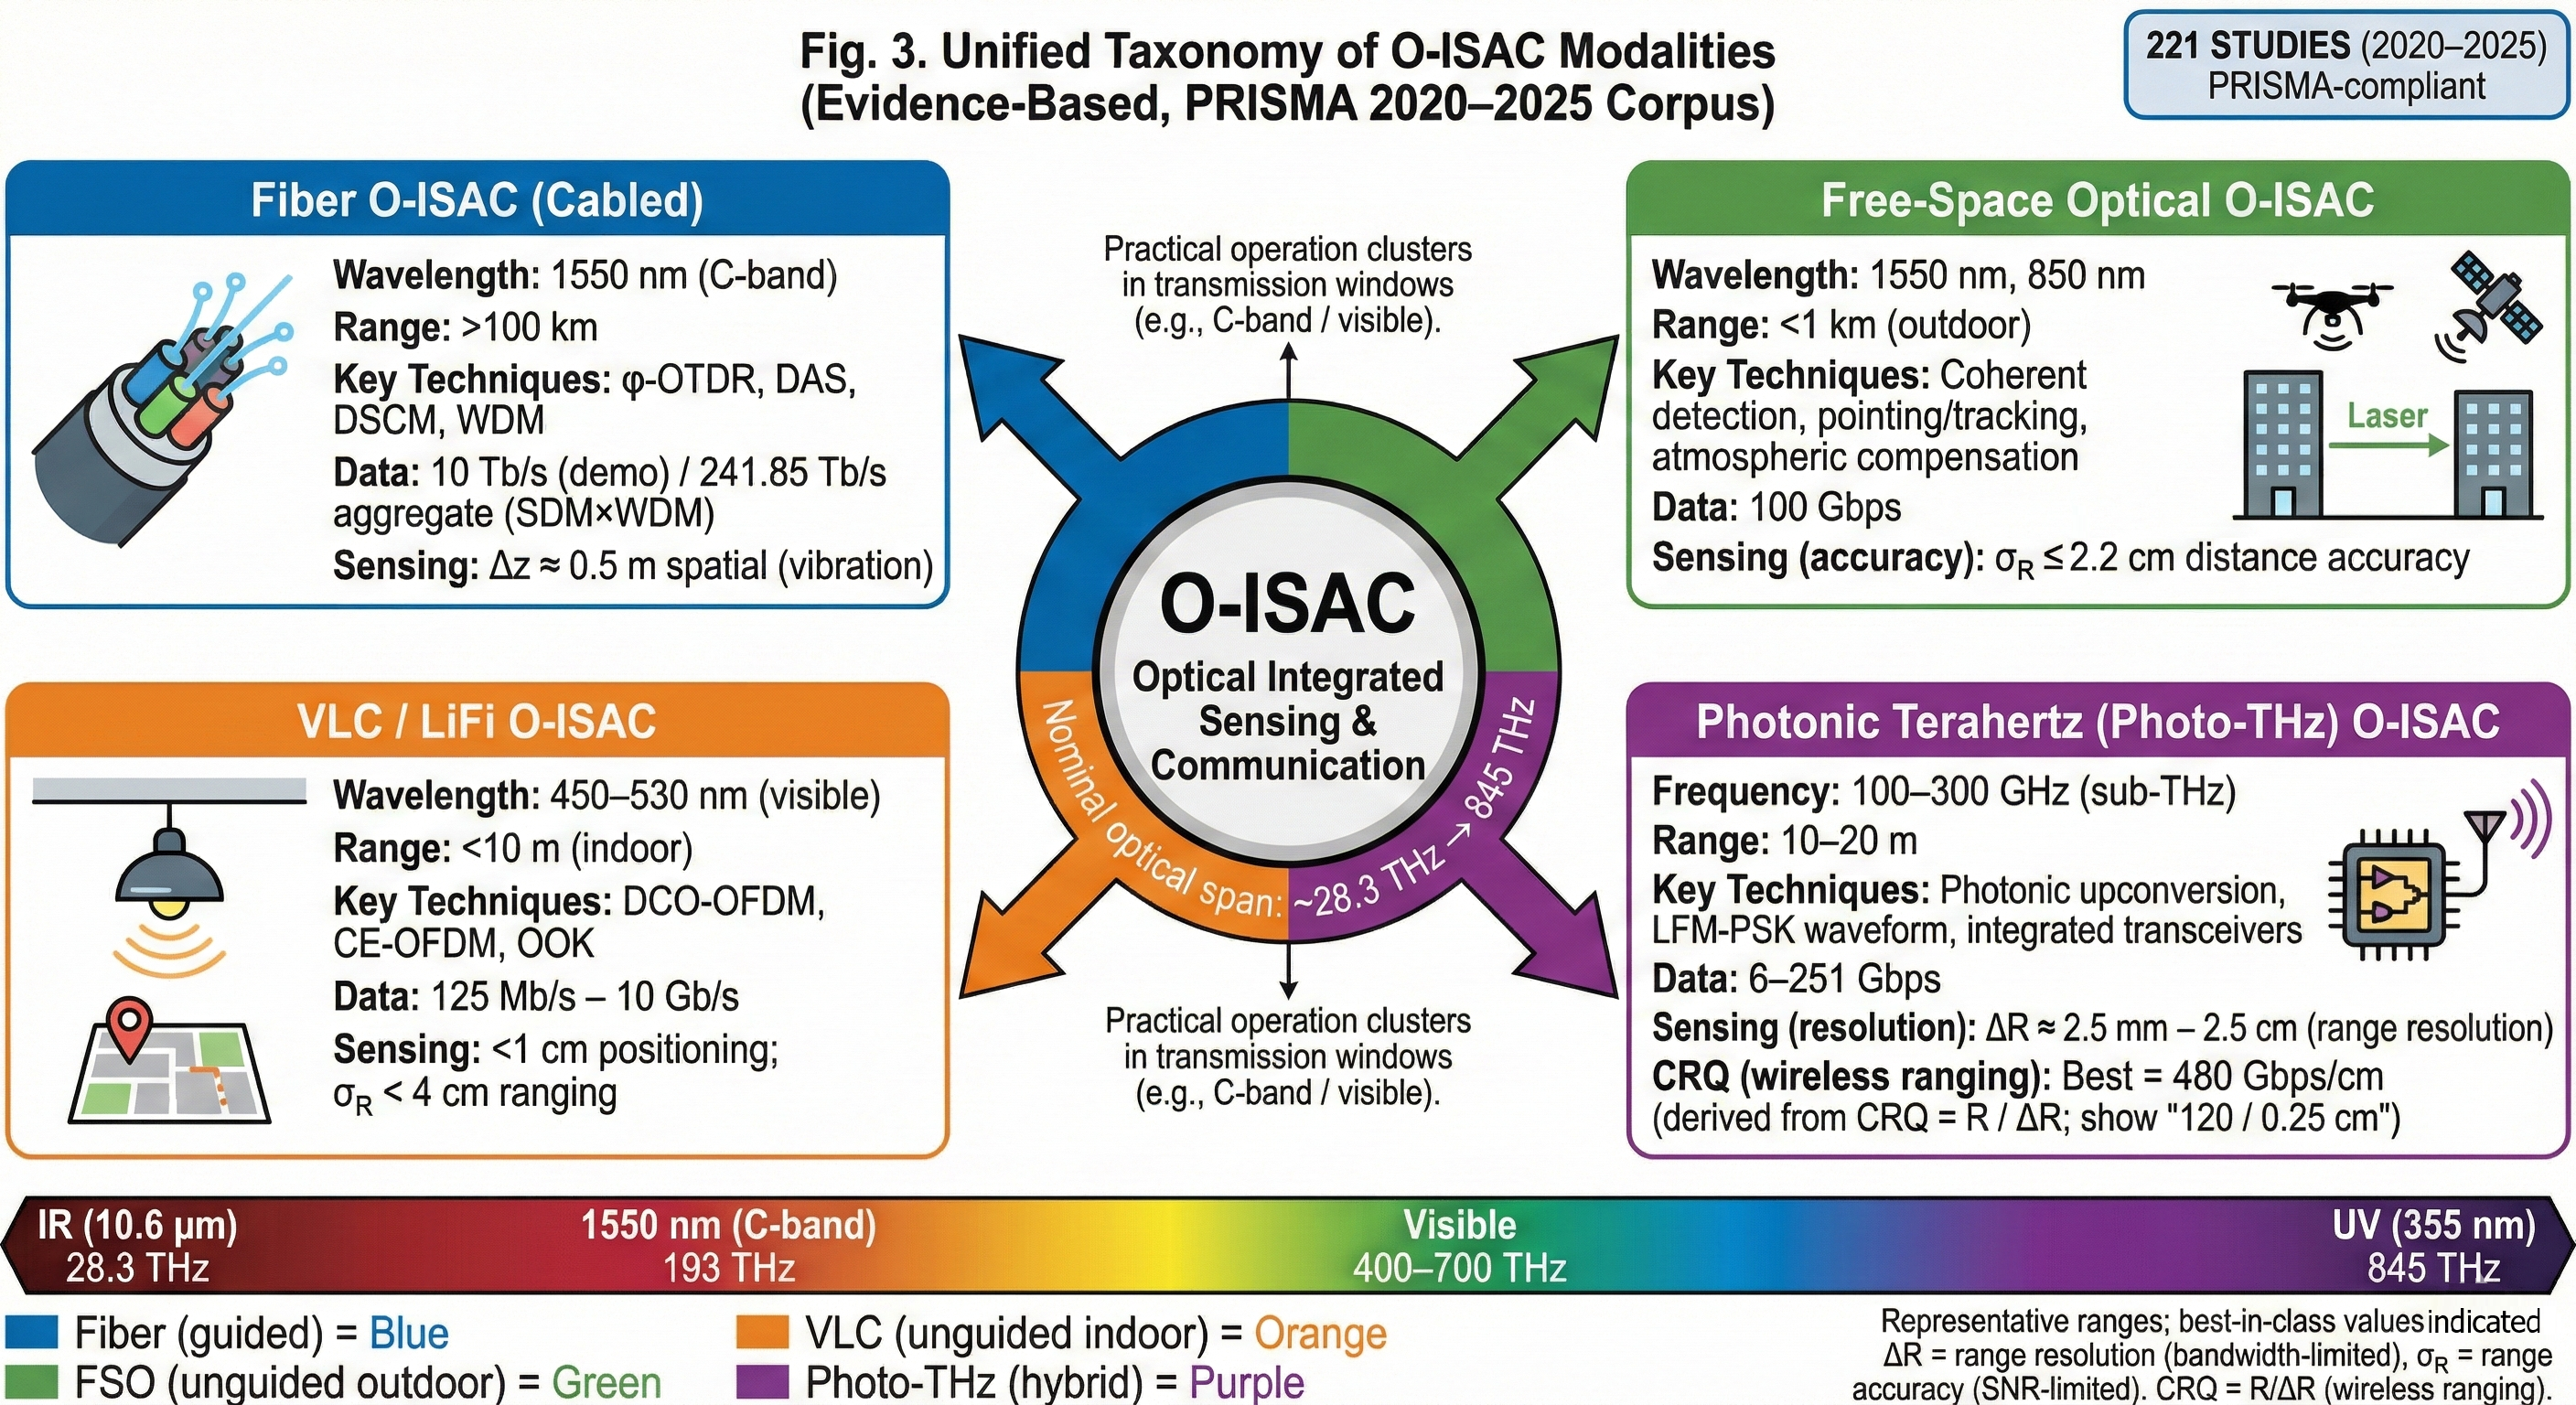
\includegraphics[width=\linewidth]{figures/fig3.png}
    \caption{The unified taxonomy of O-ISAC modalities derived from a systematic PRISMA-compliant analysis of 220 primary studies (2020--2025). (Top-Left) Fiber O-ISAC (Cabled) leveraging existing DAS/DSCM infrastructure for long-haul ($>100$ km) sensing and Tb/s-scale data transmission. (Top-Right) Free-Space Optical (FSO) O-ISAC for outdoor inter-building links utilizing coherent detection and atmospheric compensation. (Bottom-Left) Visible Light Communication (VLC) O-ISAC for indoor environments using LED infrastructure for joint illumination, high-speed connectivity, and sub-centimeter positioning. (Bottom-Right) Photonic Terahertz (Photo-THz) O-ISAC bridging the optical and wireless THz domains to achieve the highest reported $\text{CRQ}_{\Delta}$ metrics ($>100$ Gbps/cm, i.e., $>1.0\times10^{13}$ bps/m).}
    \label{fig:fig3}
\end{figure}

\begin{enumerate}
    \item \textbf{Fiber O-ISAC (Cabled):} Integration of DAS/DFOS with coherent optical transmission over single-mode/few-mode fibers. Key techniques include $\phi$-OTDR, DSCM, and WDM-based sensing-communication multiplexing.
    \item \textbf{Free-Space Optical (FSO) O-ISAC:} Outdoor/inter-building links using 1550 nm laser transmission with atmospheric channel compensation. Achieved ranges: $<1$ km with 100 Gbps capacity.
    \item \textbf{Visible Light Communication (VLC) O-ISAC:} Indoor systems leveraging LED illumination infrastructure for simultaneous lighting, communication, and positioning. Key modulations: DCO-OFDM, CE-OFDM, OOK.
    \item \textbf{Photo-THz O-ISAC:} Photonic-assisted sub-THz (100--300 GHz) systems bridging optical generation with wireless THz transmission. This emerging modality offers the highest reported $\text{CRQ}_{\Delta}$ values ($>100$ Gbps/cm, i.e., $>1.0\times10^{13}$ bps/m) \cite{O_ISAC_016}.
\end{enumerate}

This unified taxonomy bridges the previously disjoint communities of optical communications, distributed fiber sensing, and optical wireless research---providing a coherent framework for cross-domain technology transfer. This taxonomy provides a common reference frame; however, the same modality boundaries also expose a deeper issue---terminology, metrics, and evaluation protocols remain inconsistent across communities, motivating the fragmentation challenge discussed next in Section I-C.

\subsection{The Fragmentation Challenge: A Landscape Without Unity}

Despite the compelling physical advantages outlined above, the O-ISAC research landscape remains highly fragmented. Our systematic analysis of \textbf{220 peer-reviewed O-ISAC studies (2020--2025)} reveals four intertwined manifestations of this fragmentation---(i) inconsistent terminology, (ii) non-standardized sensing metrics, (iii) siloed modality communities, and (iv) limited cross-domain technology transfer---together impeding reproducibility, cross-study comparability, and ultimately the maturation of a unified 6G optical sensing--communication framework.

\textbf{Terminology Proliferation.} A foundational barrier to synthesis is the proliferation of synonymous and near-synonymous terms for closely related concepts. For instance, a single work may frame ISAC under an umbrella of aliases such as \textit{"radar-communication (RadCom), joint radar-communication (JRC), and other related terms"} \cite{O_ISAC_161}, while VLC-centric studies describe \textit{"Joint Communication and Sensing (JCS), also known as Integrated Sensing And Communication (ISAC), [and] Sensing-Communication Integration (SCI)"} \cite{O_ISAC_068}. In the fiber community, the vocabulary further diverges into "ISAC-OF" (ISAC in optical fiber), "fiber-ISAC," and "photonic ISAC" \cite{O_ISAC_041}, \cite{O_ISAC_033}. This aliasing is not merely cosmetic: it complicates systematic discovery, inflates perceived novelty through re-labeling, and obscures conceptual linkages across modalities and hardware assumptions.

\textbf{Metric Non-Isomorphism.} Equally problematic is the absence of a shared sensing-performance language. A first-order example is the recurrent conflation of \textbf{physical resolution limits} with \textbf{estimator-dependent accuracy} and \textbf{information-/estimation-theoretic bounds}. For ranging, the bandwidth-limited (two-way) physical resolution is governed by
\begin{equation}
\Delta r_{\min}=\frac{v}{2B_{\text{eff}}},
\end{equation}
where $v=c$ in free space and $v\approx c/n_g$ in guided media (with group index $n_g$), hence representing a modality-dependent propagation speed but a common bandwidth principle. In contrast, reported "accuracy" metrics---RMSE, $\sigma_r = \sqrt{\mathbb{E}[(\hat r - r)^2]}$, or "localization error"---are inherently SNR-dependent and estimator-dependent, while CRB/FIM-based quantities characterize information-/estimation-theoretic bounds under an explicitly stated observation model \cite{O_ISAC_013}, \cite{O_ISAC_050}, \cite{O_ISAC_056}. The practical consequence is that papers can report "resolution" in incommensurate senses: fiber DAS studies may report "spatial resolution" as a minimum resolvable segment length \cite{O_ISAC_013}, whereas FSO ranging papers may report "range resolution" via bandwidth-derived definitions \cite{O_ISAC_035}. Additionally, "signal quality" is not referenced to a consistent measurement plane: coherent fiber systems often report OSNR in the optical domain \cite{O_ISAC_028}, whereas VLC systems typically report electrical SNR after photodetection \cite{O_ISAC_009}, complicating direct cross-modality comparisons without an explicit normalization convention.

\textbf{Sub-Domain Siloing and Limited Cross-Citation.} The literature has evolved along several largely independent trajectories---fiber DAS/communication co-design, FSO ranging--communication integration, VLC positioning--data links, and photonic-THz ISAC---each anchored in distinct channel models (guided vs. turbulent vs. LoS-dominated), transceiver paradigms (coherent DSP-driven optics vs. IM/DD LEDs), and evaluation benchmarks, with limited cross-pollination \cite{O_ISAC_033}, \cite{O_ISAC_050}, \cite{O_ISAC_082}. Consequently, what appears as a "trade-off frontier" in one modality is often not directly comparable to another without carefully harmonized assumptions and metrics. This siloing is echoed in recent assessments: \textit{"VLC and VLP systems are usually designed separately... mutual benefits between positioning and communication have not been utilized effectively"} \cite{O_ISAC_039}, and \textit{"interoperability and certification across sectors remain a significant barrier"} \cite{O_ISAC_161}.

\textbf{Weak Cross-Domain Technology Transfer.} Beyond vocabulary and metrics, fragmentation manifests as limited portability of methods and abstractions. Waveform and probing strategies developed in fiber-ISAC contexts (e.g., LFM-embedded training structures \cite{O_ISAC_042}, polarization-based sensing probes \cite{O_ISAC_074}) are only rarely transferred to free-space or VLC channels, while VLC-driven approaches (e.g., multi-carrier localization with m-CAP \cite{O_ISAC_022}, learning-enabled joint positioning \cite{O_ISAC_039}) seldom reappear in FSO or photonic-THz settings. Hardware constraints further impede transfer: coherent fiber transceivers rely on DSP-intensive equalization and phase-sensitive reception \cite{O_ISAC_033}, whereas IM/DD LED-based O-ISAC is amplitude-constrained and often bandwidth-limited \cite{O_ISAC_054}. In the absence of shared benchmarks and reporting protocols, it remains difficult to distinguish what is fundamentally modality-specific from what is transferable across optical platforms \cite{O_ISAC_068}, \cite{O_ISAC_067}.

\textbf{The Missing Unifying Framework.} Collectively, these issues point to a critical gap: the absence of a unified physical-layer taxonomy, a standardized performance-reporting contract, and a cross-modality benchmark suite. A minimal reporting contract should at least specify: (i) communication performance (rate, BER/FEC margin), (ii) sensing performance separated into physical resolution $\Delta r_{\min}$, estimator-level error (RMSE/$\sigma_r$), and information-/estimation-theoretic bounds (CRB/FIM), (iii) signal quality defined at an explicit reference plane (electrical SNR vs. OSNR), and (iv) channel/scenario assumptions that govern comparability. Recent calls for \textit{"a standard VLC channel model... following the modeling methodology of 3GPP"} \cite{O_ISAC_327} and for \textit{"standardization efforts for facilitating interoperability"} \cite{O_ISAC_068}, \cite{O_ISAC_082} underscore the urgency of this unification. Without such a framework, O-ISAC risks continued siloing, duplicated effort, and missed opportunities for cross-domain synergy---an observation that directly motivates the next section, where we systematically position existing surveys and identify the gaps that our PRISMA-based unified treatment addresses.

\subsection{Related Surveys and Gap Analysis}

The rapid maturation of RF-based ISAC has given rise to a well-developed survey landscape in the radio-frequency domain, where comprehensive tutorials address waveform design, beamforming strategies, and information-theoretic limits for dual-function radar-communication systems. Hardware-centric ISAC transceiver surveys (RF-oriented) provide useful background but do not address optical modalities \cite{O_ISAC_161}. In contrast, the optical ISAC domain remains comparatively underserved: existing review-style works are distributed across disjoint modality communities---VLC positioning, distributed fiber sensing, FSO channel modeling, and photonic-THz transmission---with limited cross-pollination and no unifying systematic treatment. This section maps the current landscape of related survey-style works, organized into Tier-1 (true O-ISAC surveys within our corpus) and Tier-2 (feeder/adjacent works that inform but do not unify the O-ISAC narrative), and identifies the critical gaps that motivate the present systematic review.

\textbf{VLC Positioning and Indoor Optical Surveys.} A growing body of work examines visible light communication for indoor positioning and data transmission. Studies exploring joint communication and sensing prospects through visible light highlight the potential of VLC for simultaneous high-speed data links and localization, while noting that spectrum scarcity, interference management, and hardware limitations remain significant barriers \cite{O_ISAC_068}. Channel characterization surveys for VLC-IoE applications in 6G provide detailed modeling of indoor optical propagation but focus primarily on the communication link rather than integrated sensing functionality \cite{O_ISAC_327}. Experimental works on integrated VLC positioning and communication---including 6-DoF location-and-pose estimation algorithms \cite{O_ISAC_062} and photonic W-band ISAC demonstrations \cite{O_ISAC_044}---advance individual system designs but do not consolidate findings into a unified cross-modality framework.

\textbf{Distributed Fiber Sensing and Fiber-ISAC Reviews.} In the cabled domain, distributed fiber optic sensing (DFOS) techniques---particularly $\phi$-OTDR-based distributed acoustic sensing (DAS)---have reached commercial maturity for infrastructure monitoring. Recent works addressing integrated sensing and communication in optical fiber present the current development status and representative system architectures \cite{O_ISAC_006}, while experimental demonstrations of co-route fiber recognition and status diagnosis based on ISAC principles \cite{O_ISAC_041} and high-precision vibration localization in bidirectional transmission systems \cite{O_ISAC_090} illustrate the growing interest in fiber-ISAC integration. Ultra-large dynamic vibration sensing with fronthaul analog radio-over-fiber transmission further extends the sensing--communication co-design paradigm \cite{O_ISAC_189}. However, these works remain largely anchored in fiber-specific channel models and DSP paradigms, with limited consideration of how insights might transfer to wireless optical or hybrid fiber-wireless scenarios.

\textbf{FSO Channel Modeling and Photonic-THz Surveys.} Free-space optical (FSO) and photonic-terahertz research constitutes a third cluster of related work. Conceptual overviews of optical integrated sensing and communication discuss architectures, potentials, and challenges for FSO-ISAC \cite{O_ISAC_021}, while emerging demonstrations of MIMO FSO with fiber Bragg grating sensors illustrate 6G IoT application potential \cite{O_ISAC_199}. Waveform-centric studies---including OCDM-based FMCW design for FSO ISAC \cite{O_ISAC_035} and photonic-based flexible ISAC with multiple targets detection capability \cite{O_ISAC_058}---advance signal processing techniques but do not synthesize findings across the FSO--fiber--VLC divide. In the photonic-THz domain, survey-style treatments exploring integrated waveforms for THz-ISAC systems summarize recent worldwide research efforts and extrapolate technological evolution tendencies \cite{O_ISAC_070}, complemented by demonstrations achieving 251 Gbps real-time communication with cm-scale sensing \cite{O_ISAC_016} and THz-over-fiber systems based on orthogonal chirp division multiplexing \cite{O_ISAC_077}. These works collectively highlight photonic-THz as the highest-CRQ$_{\Delta}$ modality but do not bridge to VLC or fiber sensing communities.

\textbf{True O-ISAC Surveys (Tier-1).} Within our systematic corpus of 220 studies, only one work explicitly frames optical ISAC as its primary subject: the VLC-based LiSAC review \cite{O_ISAC_303}. A separate RIS-for-ISAC survey \cite{O_ISAC_163} provides enabling-technology context but remains RF/THz-centric and is therefore treated as Tier-2 in Table I. Notably, the VLC review does not apply a systematic methodology (e.g., PRISMA) and remains anchored to a single modality rather than spanning the full fiber--FSO--VLC--photo-THz spectrum under a unified physical-layer abstraction.

\textbf{Gap Synthesis.} Within the optical-ISAC corpus considered in this review, our analysis reveals five critical gaps that distinguish the current landscape from a unified framework. First, no cross-modality, modality-agnostic taxonomy spanning fiber--FSO--VLC/LiFi--photo-THz under a single PHY abstraction is available; existing survey-style works typically remain medium-centric (e.g., \cite{O_ISAC_303} for VLC, \cite{O_ISAC_006} for fiber), often with overlapping or inconsistent definitions. Second, among the identified survey-style works in the considered corpus, PRISMA-aligned systematic methodology is not adopted; most contributions employ narrative or tutorial-style treatments that limit reproducibility and evidence-traceable synthesis. Third, metric normalization remains unresolved: no standardized reporting contract consistently separates bandwidth-limited physical resolution (e.g., $\Delta r_{\min} = v/(2B_{\text{eff}})$) from estimator-dependent accuracy (e.g., RMSE/$\sigma_r = \sqrt{\mathbb{E}[(\hat r - r)^2]}$) and information-/estimation-theoretic bounds (CRB/FIM), nor does a common convention exist for signal-quality reporting across modalities (electrical SNR after photodetection versus optical OSNR/power-budget conventions). Fourth, cross-domain technology transfer is underexplored, with limited explicit evaluation of portability of waveform/probing strategies and DSP abstractions across media (e.g., from coherent fiber sensing to FSO/VLC). Fifth, emerging enabling technologies---such as optical RIS and optical phased arrays---are treated in a fragmented, technology-centric manner rather than through a systematic synthesis of integration pathways and modality-agnostic design abstractions. Table I summarizes these limitations by comparing this review against representative Tier-1 and Tier-2 review- and survey-style works; it reports \textit{context descriptors} (Tier, modality scope, integration depth, methodology) and evaluates \textbf{five gap axes} (taxonomy, metrics, benchmarking, transfer, enablers).

These gaps collectively establish the rationale for this review: a PRISMA-compliant systematic review that unifies O-ISAC across all four modalities, establishes a standardized taxonomy and reporting contract, and synthesizes quantitative trade-off frontiers to guide future research.

\begin{quote}
\textbf{Lesson 1:} Without axis-aligned reporting (scope--taxonomy--metrics--benchmarks--transfer), the existing survey landscape cannot be converted into a defensible cross-modality O-ISAC research gap.
\end{quote}

\subsection{Contributions of This Review}

To close the five gaps identified in Section I-D, we provide evidence-backed contributions grounded in the PRISMA corpus and extraction schema; each item includes a compact Contribution-Gap-Section mapping:

\begin{enumerate}
    \item \textbf{PRISMA evidence base and quality scoring (Gap 2):} We apply the PRISMA 2020 protocol \cite{PRISMA2020} to a unified corpus of 220 studies with bibliographic year metadata available for 219 records (210 in 2020-2025), and we report complete 5-dimension TQAF scores for 208 studies. \textit{Contribution-Gap-Section:} Gap 2 $\rightarrow$ Section III.
    \item \textbf{Cross-modality taxonomy with measured coverage (Gap 1):} We construct a unified taxonomy spanning fiber, FSO, VLC/visible-light, photo-THz, and hybrid O-ISAC; the extracted medium labels include 46 fiber, 19 FSO, 26 VLC/visible-light/UV, 1 photo-THz, and 116 hybrid studies (optical-THz bridging can appear under hybrid depending on the extraction label ontology). \textit{Contribution-Gap-Section:} Gap 1 $\rightarrow$ Section IV.
    \item \textbf{Standardized reporting contract and trade-off synthesis (Gap 3):} We normalize reporting using $\Delta r_{\min}$, $\sigma_r$, and $\text{CRQ}_{\Delta}$ and quantify coverage: 217 studies report data-rate metrics, 213 report a resolution-type metric ($\Delta r_{\min}$ in ranging or $\Delta z$/spatial granularity in fiber), 208 report $\sigma_r$, and 171 report CRB/CRLB values; 213 studies report both rate and a resolution-type metric, enabling $\text{CRQ}_{\Delta}$ comparisons where $\Delta r_{\min}$ is available (N\_rate\_and\_resType = 213; N\_rate\_and\_Drmin = 160). \textit{Contribution-Gap-Section:} Gap 3 $\rightarrow$ Section V.
    \item \textbf{Enabler-centric synthesis across optical platforms (Gap 5):} We quantify enabling-technology prevalence to ground Section VI, including machine learning (53 studies), optical RIS (ORIS, 8 studies), and optical phased arrays (OPA, 7 studies), and relate these tags to the integration pathways discussed in the enabler section. \textit{Contribution-Gap-Section:} Gap 5 $\rightarrow$ Section VI.
    \item \textbf{Cross-domain transfer map tied to applications (Gap 4):} We build a modality-application transfer map in Section VII; 15 application domains appear in $\ge$2 modality classes (8 domains in $\ge$3), with high-frequency domains including industrial manufacturing (65), vehicular (60), indoor positioning (56), and 6G networking (46). \textit{Contribution-Gap-Section:} Gap 4 $\rightarrow$ Section VII.
\end{enumerate}

\begin{quote}
\textbf{Lesson 2:} A systematic, PRISMA-based methodology enables reproducible evidence synthesis and uncovers research gaps that are invisible in narrative reviews.
\end{quote}

\subsection{Organization of This Paper}

The remainder of this review is organized as follows:

\begin{itemize}
    \item \textbf{Section II (Technical Fundamentals)}: Provides the physical-layer foundations of optical sensing and communication, covering modulation schemes, channel models, and hardware architectures.
    \item \textbf{Section III (Methodology)}: Details the PRISMA 2020-compliant systematic review methodology, including search strategy, eligibility criteria, study selection process, and the 5-dimensional Technical Quality Assessment Form (TQAF).
    \item \textbf{Section IV (Unified O-ISAC Taxonomy)}: Presents the proposed cross-domain taxonomy, organizing 220 studies by medium, integration mechanism, and signal dimension.
    \item \textbf{Section V (Performance Trade-off Analysis)}: Synthesizes quantitative performance metrics to characterize rate-resolution trade-offs and Pareto-optimal operating regions.
    \item \textbf{Section VI (Enabling Technologies)}: Analyzes key enabling technologies including ORIS, OPA, photonics-assisted signal generation, and machine learning integration.
    \item \textbf{Section VII (Applications and Use Cases)}: Synthesizes representative use cases across smart infrastructure (including industrial IoT motifs), indoor environments (including healthcare-oriented motifs), automotive transportation, underwater/subsea monitoring, and space/satellite networks, and then consolidates cross-domain transfer in VII-F with dual-view consistency analysis in VII-G.
    \item \textbf{Section VIII (Open Challenges and Research Roadmap)}: Synthesizes five challenge domains, organizes a capstone dependency-aware research agenda toward 6G integration, and closes with a cross-section alignment audit that verifies continuity with Sections V-VII.
    \item \textbf{Section IX (Conclusions)}: Summarizes the key findings and provides closing remarks.
\end{itemize}

\subsection{Notation and Acronyms}

For the reader's convenience, the mathematical notation conventions and the most frequently used acronyms in this paper are defined in Tables III and IV, respectively.

\begin{table}[htbp]
\caption{Mathematical Notation Conventions}
\label{tab:math_notation}
\centering
\setlength{\tabcolsep}{4pt}
\renewcommand{\arraystretch}{1.1}
\begin{tabularx}{\textwidth}{@{}L{4.8cm}Y@{}}
\toprule
\thead{Symbol} & \thead{Definition} \\
\midrule
$\lambda$ & Optical wavelength (nm) \\
$B_{\text{eff}}$ & Effective signal bandwidth (Hz) \\
$R$ & Data rate (bit/s) \\
$d$ & Target distance/range (m) \\
$\Delta r_{\min}$ & Bandwidth-limited (two-way) range resolution (m) \\
$\sigma_r = \sqrt{\mathbb{E}[(\hat r - r)^2]}$ & Range estimation error / RMSE (m) \\
$\text{SNR}$ & Signal-to-noise ratio \\
$\text{BER}$ & Bit error rate \\
$\alpha$ & Power allocation factor (C\&S trade-off) \\
\bottomrule
\end{tabularx}
\end{table}

\begin{table}[htbp]
\caption{List of Frequently Used Acronyms}
\label{tab:acronyms}
\centering
\setlength{\tabcolsep}{4pt}
\renewcommand{\arraystretch}{1.08}
\begin{tabularx}{\textwidth}{@{}L{2.8cm}Y@{}}
\toprule
\thead{Acronym} & \thead{Definition} \\
\midrule
\textbf{ISAC} & Integrated Sensing and Communication \\
\textbf{O-ISAC} & Optical Integrated Sensing and Communication \\
\textbf{ISAC-OF} & Integrated Sensing and Communication in Optical Fiber \\
\textbf{DFS} & Distributed Fiber Sensing \\
\textbf{DAS} & Distributed Acoustic Sensing \\
\textbf{VLC} & Visible Light Communication \\
\textbf{FSO} & Free-Space Optical \\
\textbf{OWC} & Optical Wireless Communication \\
\textbf{LFM} & Linear Frequency Modulation \\
\textbf{OFDM} & Orthogonal Frequency Division Multiplexing \\
\textbf{DCO-OFDM} & DC-biased Optical OFDM \\
\textbf{OCDM} & Orthogonal Chirp Division Multiplexing \\
\textbf{IM/DD} & Intensity Modulation / Direct Detection \\
\textbf{ORIS} & Optical Reconfigurable Intelligent Surface \\
\textbf{OPA} & Optical Phased Array \\
\textbf{PIC} & Photonic Integrated Circuit \\
\textbf{CCR} & Corner Cube Reflector \\
\textbf{RO-ISAC} & Retroreflective O-ISAC \\
\textbf{$\phi$-OTDR} & Phase-Sensitive Optical Time-Domain Reflectometry \\
\textbf{SMF} & Single-Mode Fiber \\
\textbf{FMF} & Few-Mode Fiber \\
\textbf{MCF} & Multi-Core Fiber \\
\textbf{WDM} & Wavelength Division Multiplexing \\
\textbf{DSCM} & Digital Subcarrier Multiplexing \\
\textbf{THz} & Terahertz \\
\textbf{MIMO} & Multiple-Input Multiple-Output \\
\textbf{PRISMA} & Preferred Reporting Items for Systematic Reviews and Meta-Analyses \\
\textbf{TQAF} & Technical Quality Assessment Form \\
\textbf{RMSE} & Root Mean Square Error \\
\textbf{CRB} & Cram\'er-Rao Bound \\
\bottomrule
\end{tabularx}
\end{table}
